% REMEMBER: You must not plagiarise anything in your report. Be extremely careful.

\documentclass{l4proj}

\usepackage{amsmath}
\usepackage{amssymb}

\newcommand{\cit}[1]{(\cite{#1})}
\newcommand{\scoreeqn}{\[S(C|T) = \sum_{A \in T}{ln\left(\dfrac{
												    P(A) + c\cdot ({I_{A, M}}^\eta + x\cdot {P(A)})
												    }{P(A)\cdot(1 + c \cdot (\sum_{A \in \mathbb{A}}{({I_{A, M}}^\eta} + x))
												    }\right)}\]}

\begin{document}

%==============================================================================
%% METADATA
\title{Pep2Path v2}
\author{Ross McBride}
\date{}

\maketitle

%==============================================================================
%% ABSTRACT
\begin{abstract}
\end{abstract}

%==============================================================================

% EDUCATION REUSE CONSENT FORM
% If you consent to your project being shown to future students for educational purposes
% then insert your name and the date below to  sign the education use form that appears in the front of the document. 
% You must explicitly give consent if you wish to do so.
% If you sign, your project may be included in the Hall of Fame if it scores particularly highly.
%
% Please note that you are under no obligation to sign 
% this declaration, but doing so would help future students.
%
%\def\consentname {My Name} % your full name
%\def\consentdate {20 March 2018} % the date you agree
%
\educationalconsent


%==============================================================================
\tableofcontents

%==============================================================================
%% Notes on formatting
%==============================================================================
% The first page, abstract and table of contents are numbered using Roman numerals and are not
% included in the page count. 
%
% From now on pages are numbered
% using Arabic numerals. Therefore, immediately after the first call to \chapter we need the call
% \pagenumbering{arabic} and this should be called once only in the document. 
%
% The first Chapter should then be on page 1. You are allowed 40 pages for a 40 credit project and 20 pages for a 
% 20 credit report. This includes everything numbered in Arabic numerals (excluding front matter) up
% to but excluding the appendices and bibliography.
%
% You must not alter text size (it is currently 10pt) or alter margins or spacing.
%
%
%==================================================================================================================================
%
% IMPORTANT
% The chapter headings here are **suggestions**. You don't have to follow this model if
% it doesn't fit your project. Every project should have an introduction and conclusion,
% however. 
%
%==================================================================================================================================
\chapter{Introduction}

% reset page numbering. Don't remove this!
\pagenumbering{arabic} 

One particular problem of interest for biologists is the identification of new biological products with novel properties. Until relatively recently, this process was done manually by trained experts. But with the recent advent of the field of bioinformatics, we can now bring immense computational resources to bear on problems like this, saving precious expert time.

Pep2Path \cit{p2p} is a tool that aims to accelerate drug identification by matching mass-spectrometry outputs to identified biosynthetic gene clusters and in the original paper the authors demonstrate robust benchmarking results. However, despite the utility of Pep2Path, it is implemented as a few monolithic scripts, with little room to revise elements of it in accordance with new developments and research without a complete rewrite. In this paper we present a small suite of software tools implementing a platform for functionality like Pep2Path, and the software process by which this software was designed and created.

\section{Aims}

The aims of the project are to:

\begin{itemize}
\item Implement a set of software tools that can achieve similar functionality to the original Pep2Path, subject to correctness testing.
\item Achieve a degree of flexibility in the implementation such that this software can be responsively updated to changes in its environment.
\item Follow good software practises in the implementation such as loose coupling such that we can achieve software reuse, a cornerstone of software development.
\end{itemize}

\section{Motivation}

Various biological compounds, are formed from assembly-chains of smaller compounds, such as peptides, formed from amino acids.
If we look at this problem as a computer scientist might, the first thing to come to mind in identifying useful drugs within this space might be an exhaustive search of all combinations of molecule.
(Of course, for other molecules questions of topology and structure come into question...)
This quite quickly runs into problems, as with the addition of each component to a chain of biological molecules, the chemical space grows exponentially.
For example, if we consider the relatively limited case of the twenty proteinogenic amino acids and a peptide of length 4, there are \(20^4\) possible combinations... Around 160,000! We would then have to identify which, if any, of these have useful properties.

Without some heuristic (for example being able to infer properties from chemical composition), an exhaustive search of the chemical space is impossible.
Instead we identify biological products produced in the wild, by living organisms - so-called 'natural products'.
From an evolutionary perspective, we expect that if organisms are expending resources on producing a particular biological product, then it confers a survival advantage.
For example, a strain of bacteria might produce an antibiotic that kills another competitor species of bacteria - which we can then use ourselves to kill a potentially deadly strain of bacteria.
Natural products produced in this way to fulfil an auxiliary function not directly related to the growth or reproduction of the organism are known as 'secondary metabolites'.

To identify potentially interesting natural products we could, for example, analyse chemical structure for similarity to other interesting compounds, or by observing similar behaviour across several species which produce a particular product. 
However, we also want to match this natural product to the gene cluster - a Biosynthetic Gene Cluster, henceforth BGCs - which encodes it.
One way of achieving this is to cluster together species that share a BGC and produce the natural product in question - this is a good indication that the pattern is meaningful and the BGC produces the natural product.

Mass spectrometry allows us to identify the chemical composition of compounds - by breaking up molecules and then measuring the mass lost, we can infer the \textit{potential} composition of a compound by the masses of its components using a mass-translation table. Mass spectrometry readings, or amino acid sequences, are one of the key inputs to Pep2Path, which provides two algorithms, for two different natural product classes: Non-Ribosomal Peptides (henceforth NRPs) and Ribosomally-synthesized and Post-translationally-modified Peptides (henceforth RiPPs). 

The other key input to each of the two Pep2Path algorithms is the gene sequence we are attempting to match our compound to. As their name suggests, RiPPs are synthesised by ribosomes, the cell organelle responsible for translating gene sequences to proteins (peptides made up of the 20 proteinogenic amino acids) and then modified post-translation by enzymes. As a result, they are directly encoded directly in an organism's gene sequence and and we can retrieve their composition directly, as Pep2Path does by obtaining their 'six translation frames'. NRPs, by contrast, are instead synthesised by Non-Ribosomal Peptide Synthetases (henceforth NRPSes) which are independent of the ribosome and can introduce non-proteinogenic amino acids. These consist of several NRPS modules which form an assembly-line of amino acids, and are controlled by three domains - A (Adenylation), T (Thiolation) and C (Condensation). Of particular interest to us is the Adenylation domain, which controls which substrate is added to the chain of amino acids. These are not directly encoded into the gene, and therefore harder to predict, and we rely on an external tool, antiSMASH \cit{as4} for this purpose.

Taking these two sets of inputs, NRP2Path matches the potential chemical compositions generated by mass spectrometry analysis to BGC predictions using antiSMASH, whereas RiPP2Path matches these potential chemical compositions to the six-frame translation extracted from the genetic sequence data of the RiPP-producing BGCs. Pep2Path can then automatically score these two sets of data against one another, filling a key part in an automated drug-identification pipeline, where previously investigation of natural products would be based on hand-identification.

However, the original Pep2Path is written almost entirely using singular scripts, one for each algorithm, with some custom data formats and some miscellaneous extra files. As a result, it breaches some important software design principles, by mixing concerns such as parsing input and generating sequence tags, and at times relies on data structures passed around the entire script. This design makes Pep2Path difficult to update, but there are a number of reasons why it might be advantageous to do so. For one, the scoring method the authors use is based on antiSMASH 2.0 \cit{as2} the current version at the time. Since the release of Pep2Path, there have been antiSMASH versions up to 4. \cit{as4} While the original Pep2Path scoring method is backwards-compatible, antiSMASH version 4.0 offers the SANDPUMA ensemble algorithm \cit{sandpuma} which collates the Stachelhaus Code and SVM predictors that antiSMASH 2.0 uses along with several others to offer a more accurate BGC prediction.

Furthermore, we may want to investigate product classes other than NRPS and RiPP, the classes of biological product on which Pep2Path operates - there are many others, including polyketides and alkaloids. (For an example as to why this might be useful, the pain-medication morphine is an alkaloid extracted from the opium poppy.) It would also be useful to integrate different algorithms for identifying biological products from sequence data such as the RiPPQuest \cit{rippq} method for lanthipeptides (a subtype of RiPP), decouple the mass spectrometry process from the Pep2Path process or otherwise update the scoring mechanism with new developments. We also expect more generally that having a more transparent and modular software design might lead to easier discovery of bugs or integration with other codebases.

%==================================================================================================================================
\chapter{Background}

\section{Mass Spectrometry}

\section{BGC Substrate Detection}

\subsection{NRPS and antiSMASH}

antiSMASH (antibiotics and Secondary Metabolite Analysis Shell) \cit{as4} is a widely-used piece of bioinformatics software used for the automated labelling of BGCs and geonome-mining of secondary metabolites from raw sequence geonome sequence data extracted from bacteria, fungi or plants. It is usable both as a standalone program on MacOS or Linux and as a web-server and has gone through several revisions and is, at the time of writing, currently up to version 4.0. Therefore, it aggregates many of the latest developments in natural product research and offers many features for the handling of such sequence data and the annotation of its BGCs, outputting data in the standard GenBank format.

For the purposes of this paper, we are interested in antiSMASH's ability to predict the substrate specificity of an NRPS' adenylation domains, that is, give us a prediction for the chemical makeup of a particular NRP given the sequence data of the organism that produces it. The current version of antiSMASH uses the SANDPUMA ensemble algorithm to do this, which aggregates the results of several other predictive algorithms, including those in previous versions of antiSMASH (maintaining backwards-compatibility), to produce significantly better results. However SANDPUMA and antiSMASH 4.0 are relatively recent compared to Pep2Path, and instead we are interested in two key predictors of antiSMASH 2.0: the Stachelhaus Code, a set of rules for comparing different adenylation domains created from empirical observation \cit{stachelhaus} and a machine learning Support Vector Machine (SVM) based method.

Machine learning is frequently used in bioinformatics to extrapolate underlying trends from the vast quantities of data, learning from a provided dataset useful understandings of programmer-selected features by performing some optimisation task. SVMs in particular are a classifier (that is, assign inputs to one of a set of discrete classes, in this case a substrate prediction) and attempt to draw a decision boundary separating those classes so as to minimise the distance between a certain number of the training datapoints plotted in a hyperplane. The SVM implementation for antiSMASH is provided by NRPSPredictor2, \cit{nrps2} a standalone piece of software which has since been integrated into the antiSMASH pipeline. One of the the things that makes the original Pep2Path results robust is that it was tested on datasets NRPSPredictor2 had \textit{not} been trained on, avoiding the introduction of bias and showing the generalisability of the Pep2Path method.

\subsection{RiPPs, their six-frame translation and RiPPQuest}

\section{Pep2Path}

\scoreeqn

\begin{figure}
    \centering
    \makebox[\linewidth][c]{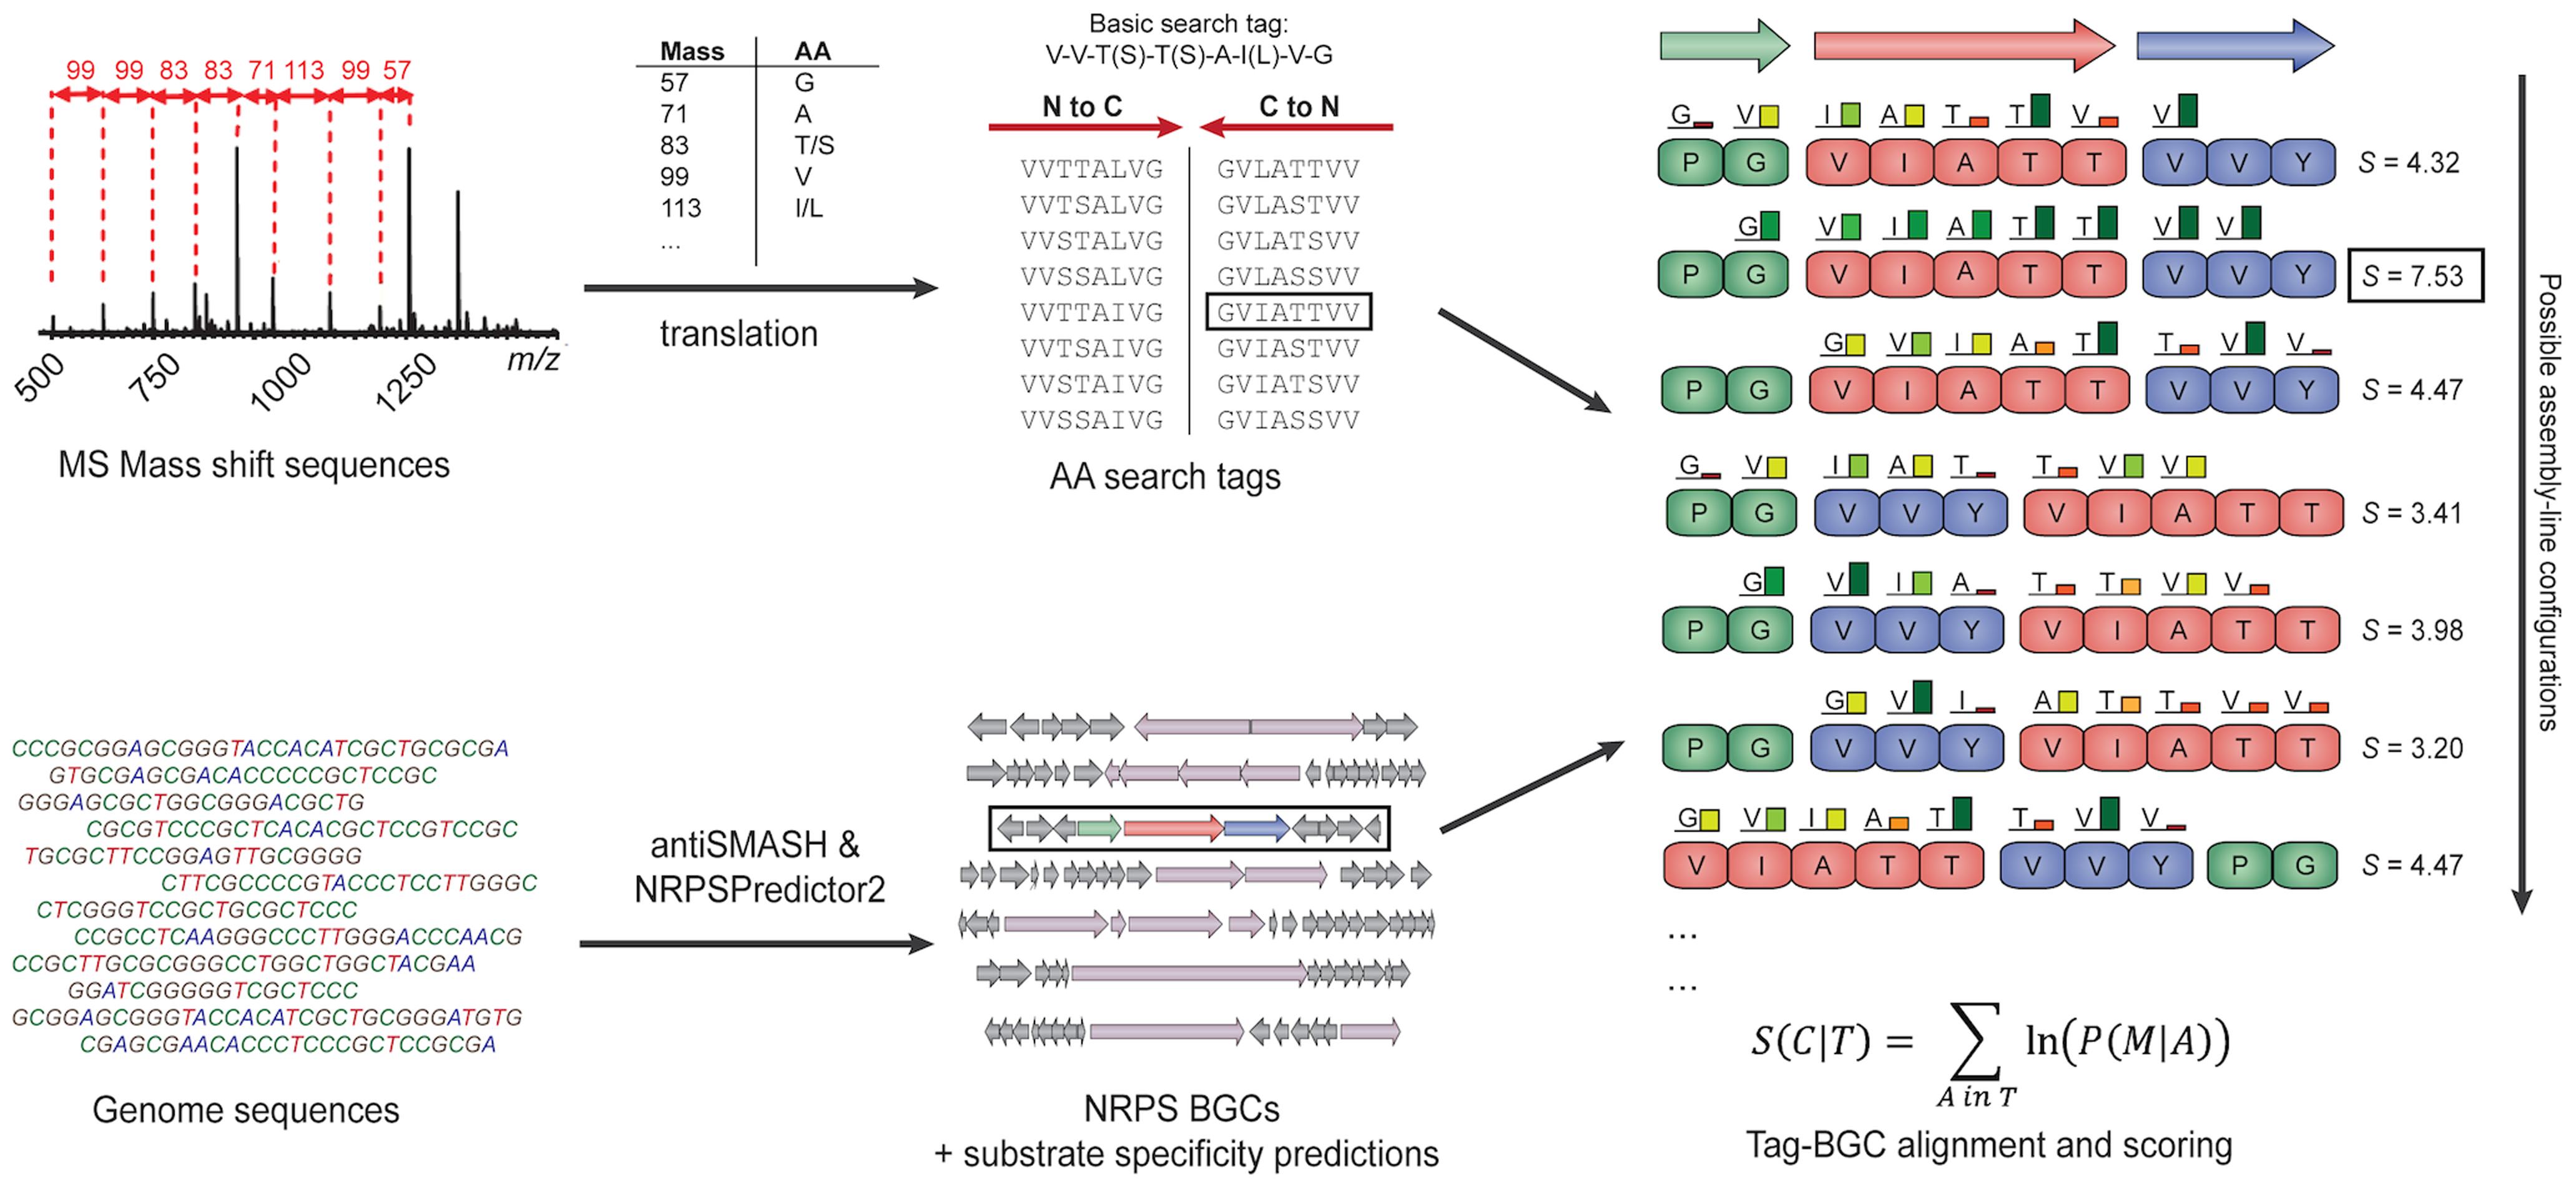
\includegraphics[width=1.25\linewidth]{images/nrp2path.png}}%

    \caption{An illustration of the NRP2Path algorithm. On the top is a mass spectrometry output being put through a mass translation table to produce
    a comprehensive list of potential sequence tags. On the bottom is BGC substrate specificity being extracted from raw sequence data by antiSMASH.
    These two sets of data are then used to compare every alignment of every sequence tag to every possible ordering of NRP blocks extracted from the 
    BGC. using the abbreviated scoring function shown below. Figure adapted from the publicly-available Pep2Path paper and online documentation.
    }

    \label{fig:nrp2path} 
\end{figure}

%==================================================================================================================================
\chapter{Analysis/Requirements}

%==================================================================================================================================
\chapter{Design}

%==================================================================================================================================
\chapter{Implementation}

%==================================================================================================================================
\chapter{Evaluation} 

%==================================================================================================================================
\chapter{Conclusion}    

%==================================================================================================================================
%
% 
%==================================================================================================================================
%  APPENDICES  

\begin{appendices}

\chapter{Appendices}

\end{appendices}

%==================================================================================================================================
%   BIBLIOGRAPHY   

% The bibliography style is abbrvnat
% The bibliography always appears last, after the appendices.

\bibliographystyle{abbrvnat}

\bibliography{l4proj}

\end{document}
